\chapter{Sample}

This is just a sample LaTeX template. \cite{YB}

\section{First section}

There are enumerations

\begin{enumerate}
    \item one
    \item two
    \item three
\end{enumerate}

But also unordered lists:

\begin{itemize}
    \item Evolution Strategies
    \item Grammatical Evolution
    \item Learning Classifier System
\end{itemize}

And we can add chapter information to our quotes.

\cite[Kap. 1.2]{Bro11} \\

\subsection{images}

We can reference to images like this: \ref{fig:sample}

\begin{figure}[h!]
    \centering
    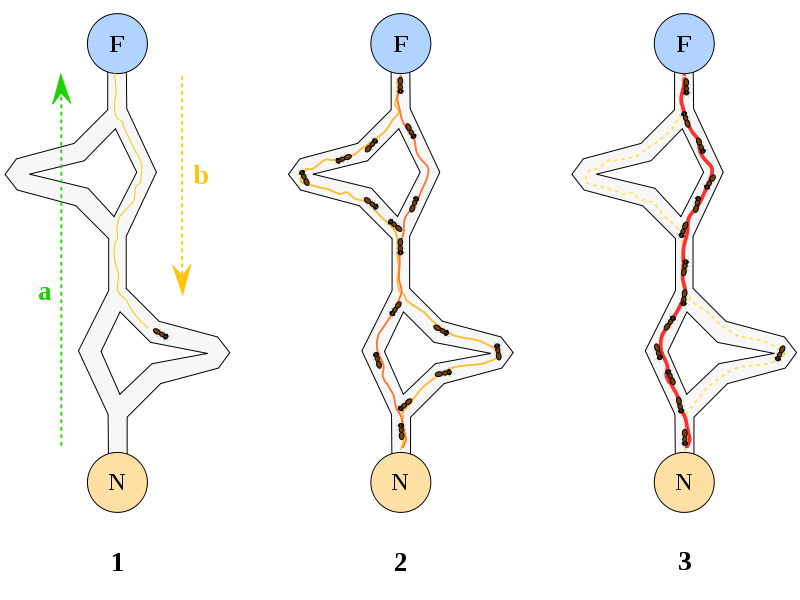
\includegraphics[scale=0.5]{resources/sample.png}
    \caption{this is some sample image \cite{YB}}
    \label{fig:sample}
\end{figure}

\subsection{code}
Die Approximation beschreibt meist eine Funktion $f$, welche möglichst nahe an eine Zielfunktion angenähert werden
möchte. Die approximierte Funktion $f$ wird aus einem Set an Beobachtungen\footnote{oftmals auch als $training$ $set$ aus
der Data Science bekannt} generiert. Solche Annäherungen werden häufig für Image Recognition verwendet
und spielen ebenfalls eine wichtige Rolle bei der Klassifikation und dem Clustering von grossen Datenmengen.